\section{Phase 4: Court Judgment Prediction}
\label{sec:phase4}

\subsection{Task and evaluation protocol}

The task assigns one of two outcome labels to each judgment in the course's
\path{Phase_4_CJPE} dataset. The primary metric is
$\mathrm{MacroF1}=(F_{1,0}+F_{1,1})/2$. The official test contains 1,517
judgments with hidden labels. Internal validation selected the checkpoint and
classification threshold. The clean development set served as a separate local
evaluation. A valid submission contains a single root-level
\path{prediction.json} with one string case ID and one binary integer prediction
per test judgment.

\begin{table}[htbp]
\centering\small
\caption{Rows, unique judgments and document lengths in the original files.
Word statistics describe rows before case-level deduplication.}
\label{tab:p4-data}
\begin{tabular}{lrrrrr}
\toprule
Split & Rows & Unique IDs & Median words & 95th percentile & Maximum words \\
\midrule
Train & 37,387 & 32,305 & 2,192 & 9,195 & 412,606 \\
Dev   & 1,988  & 994    & 2,822 & 9,280 & 42,198 \\
Test  & 1,517  & 1,517  & 2,940 & 10,023 & 40,487 \\
\bottomrule
\end{tabular}
\end{table}

The case audit found repeated IDs in 5,082 training cases and 994 development
cases. Those repeated IDs had identical normalized text and consistent labels.
The pipeline keeps the longest available text per ID with stable tie handling.
It removes development rows that share an ID or a lowercase, whitespace-normalized
text hash with test. The saved audit found zero such overlaps. A ten-fold
stratified group split (seed 42) grouped identical texts and selected the fold
closest to a 10\% holdout and the original positive-class proportion. This
yielded 29,074 training and 3,231 internal validation cases, each with about
41.4\% class 1. Clean development has 497 cases per class. A constant-class
predictor obtains 0.5000 accuracy and 0.3333 macro-F1 on that split.

\subsection{Representations and experimental design}

The tokenizer is the original 32,000-token Phase-1 byte-level BPE. The single
window retains the last 1,022 content tokens with BOS and EOS and right-padding
to at most 1,024 tokens. Tail sampling prioritizes the portion of the judgment
where dispositions may appear. It can omit facts, precedent, or procedural
context earlier in a long document. A head-and-tail representation was
prepared and checked. All eight trained runs used the tail or hierarchical
representation, so no separate head-and-tail score is available.

\begin{description}[leftmargin=1.4em]
\item[E01.] Full fine-tuning of the 700,047,360-token Efficient GQA
  foundation (14 blocks, 768 hidden units, 12 query and 4 key/value heads).
  A dropout and linear head classify the final non-padding state. The
  resulting model has 112,680,194 parameters.
\item[E02.] Up to five evenly spaced windows, always including the tail, are
  encoded with frozen E01 weights. Their final-token vectors and logits are
  cached in float16. A position-aware attention head pools chunk vectors.
  Its learned correction uses the pooled vector, tail vector, and their
  difference, then adds two residual logits to the original tail logits.
  The zero-initialized final layer starts at the frozen tail decision.
\item[E03.] Output-space multiplicative LoRMA+ with rank 16 and scale
  $\alpha/r=32/16$ in the four GQA projections and three SwiGLU projections
  per block. The pretrained matrix remains frozen and the adapter adds
  $(\alpha/r)BA(W_0x)$ to its output before bias.
\item[E04--E06.] Full tuning of the original 100,024,320-token causal decoder,
  Prefix-LM, and encoder--decoder. The decoder pools the final non-padding
  state. Prefix-LM exposes the whole valid prefix bidirectionally and masks
  padding. The encoder--decoder uses one BOS decoder query over masked
  encoder memory, with padding excluded from encoder and cross-attention.
\item[E07.] Adaptive-rank GQA freezes the same 700M foundation and adapts
  56 attention projections with a masked rank-16 factorization. An
  exponential moving average of gradient sensitivity guides irreversible
  pruning every 40 optimizer updates. The cubic budget schedule targets
  mean rank 8 with at least 2 active components per projection. The
  archived run decreased from 896 to 448 active components.
\item[E08.] A six-layer causal Transformer (384 hidden units, six heads,
  23,329,538 parameters) learns from E01 logits and the true labels.
  The objective is $0.35\,\mathrm{CE}+0.65\,T^2
  \mathrm{KL}(p_{\mathrm{teacher},T}\Vert p_{\mathrm{student},T})$ with $T=2$.
  This is about a 4.83-fold reduction in parameters relative to E01.
\item[E09--E10.] Probability blends pair E01 with E05 and E08 respectively.
  Nine E01 weights in $[0.55,0.95]$ and 51 thresholds in $[0.25,0.75]$ are
  searched on internal validation. Both selected an E01 weight of 0.90.
\end{description}

Full tuning used AdamW with backbone and head learning rates of
$2\times10^{-5}$ and $3\times10^{-4}$, microbatches of eight, four accumulation
steps, gradient clipping at 1.0, and 6\% warmup followed by cosine decay
with a 5\% floor. Adapter and student schedules retain their recorded
run-specific rates and batch sizes. E02 trains only the residual head and
uses a constant $2\times10^{-4}$ learning rate with batch size 256. The
checkpoint criterion was internal macro-F1 at threshold 0.50. Thresholds
for single runs were then tuned on the selected checkpoint's internal
predictions, preferring the threshold closest to 0.50 on a tie.
Figure~\ref{fig:p4-history} plots pre-calibration scores. These differ
from the calibrated scores in Table~\ref{tab:p4-scores}.

\begin{figure}[htbp]
\centering
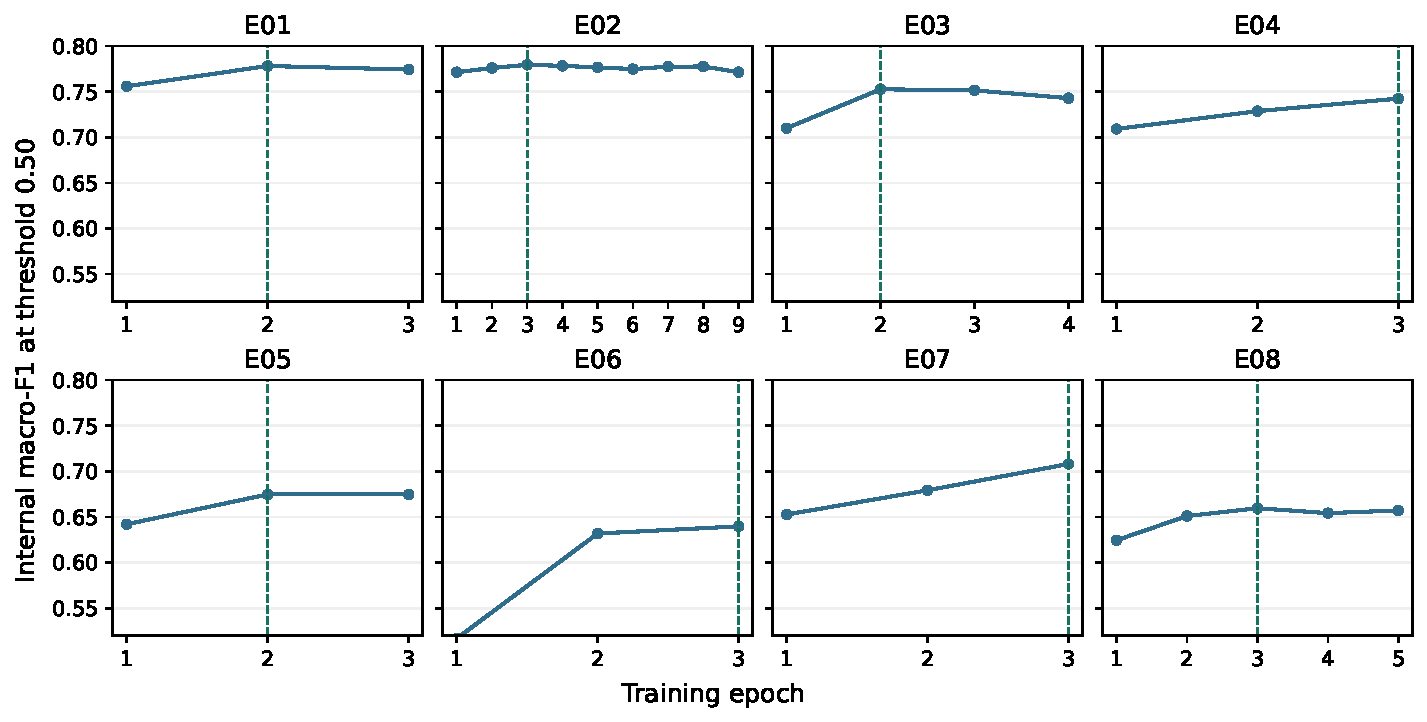
\includegraphics[width=\linewidth]{figures/phase4/p4_validation_history.pdf}
\caption{Saved epoch histories for all eight trained runs. The dashed line
marks the selected checkpoint. E02 starts from frozen E01 features, and
E08 starts from a newly initialized student, so the trajectories represent
different training regimes.}
\label{fig:p4-history}
\end{figure}

\subsection{Results and error analysis}

\begin{table}[htbp]
\centering\small
\caption{Macro-F1 by split at the selected threshold. The official scores
are supplied Codabench results. Internal and clean development scores
were recomputed from the saved outputs.}
\label{tab:p4-scores}
\begin{tabular}{llrrrr}
\toprule
Run & Experiment & Threshold & Internal & Clean dev & Codabench \\
\midrule
E01 & Efficient GQA full tuning & 0.51 & 0.7795 & 0.7328 & \textbf{0.7393} \\
E02 & Hierarchical GQA & 0.45 & 0.7809 & 0.7233 & 0.7263 \\
E03 & GQA LoRMA+ & 0.49 & 0.7548 & 0.6576 & 0.6749 \\
E04 & Decoder-only full tuning & 0.50 & 0.7423 & 0.6911 & 0.6976 \\
E05 & Prefix-LM full tuning & 0.49 & 0.6769 & 0.6445 & 0.6476 \\
E06 & Encoder--decoder full tuning & 0.46 & 0.6480 & 0.6133 & 0.6013 \\
E07 & Adaptive-rank GQA & 0.44 & 0.7150 & 0.6394 & 0.6580 \\
E08 & Distilled Transformer & 0.47 & 0.6643 & 0.6015 & 0.6126 \\
E09 & GQA + Prefix-LM & 0.48 & 0.7797 & 0.7346 & 0.7353 \\
E10 & GQA + distilled student & 0.49 & 0.7797 & 0.7329 & 0.7369 \\
\bottomrule
\end{tabular}

\end{table}

\begin{figure}[htbp]
\centering
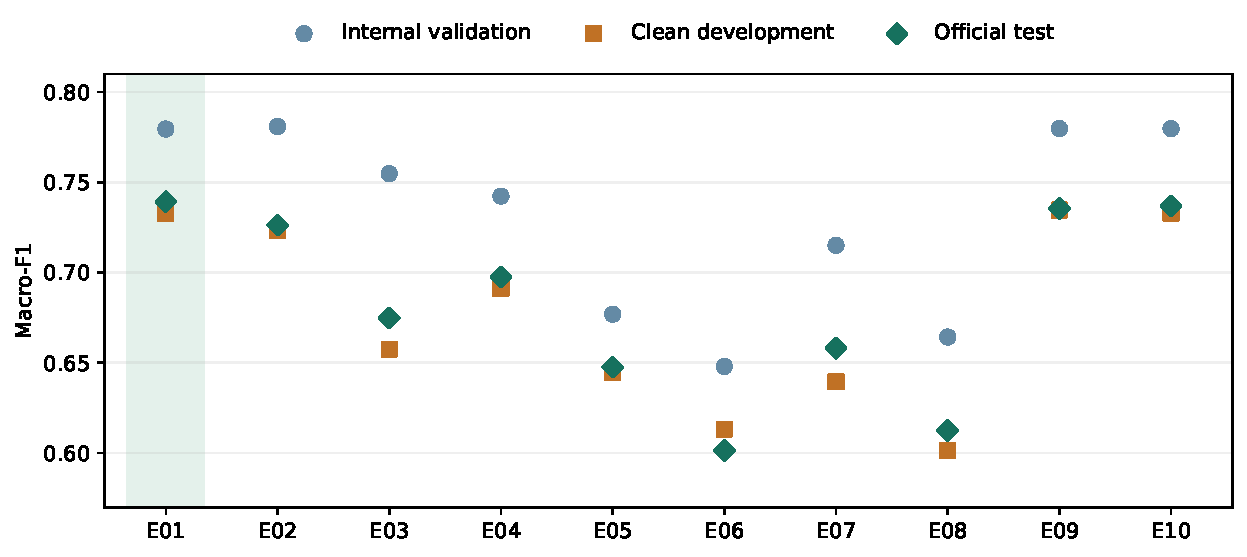
\includegraphics[width=\linewidth]{figures/phase4/p4_split_scores.pdf}
\caption{Local and official scores for all ten submissions. E02 leads on
internal validation and E09 leads on clean development. E01 leads on the
official test.}
\label{fig:p4-scores}
\end{figure}

E01 achieved the best recorded official macro-F1 of \textbf{0.7393}, ahead
of E10 (0.7369) and E09 (0.7353) by 0.0024 and 0.0040. E09 improved on E01
by 0.0018 on clean development but fell behind on the official test.
E02 improved internal macro-F1 from 0.7795 to 0.7809 while trailing E01
on both development and test. Extra document coverage and the learned
residual therefore did not yield a consistent improvement under the
observed protocol.

Among full-tuning runs, E04, E05 and E06 scored 0.6976, 0.6476 and 0.6013
officially. E01 differed in both architecture and pretraining exposure,
so the comparison cannot isolate the effect of grouped-query attention.
E03 and E07 started from the same 700M foundation as E01, but changed
the objective's trainable parameterization, optimization settings and
training schedule. E08 reached 0.6126 officially with substantially
fewer parameters. The experiment did not train a same-size supervised
student as a control, leaving the marginal effect of distillation
unmeasured.

\begin{figure}[htbp]
\centering
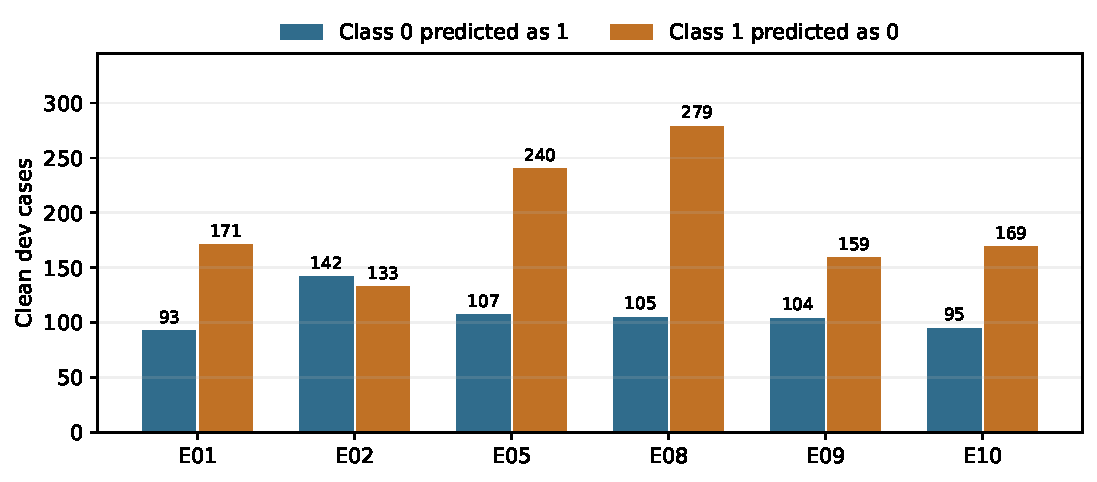
\includegraphics[width=.92\linewidth]{figures/phase4/p4_dev_errors.pdf}
\caption{Selected clean development error counts at each run's chosen
threshold. The clean split contains 497 cases per class.}
\label{fig:p4-errors}
\end{figure}

At its selected threshold E01 missed 171 of 497 class-1 cases and
classified 93 of 497 class-0 cases as class 1. E02 reduced the first
error to 133 while increasing the second to 142, a tradeoff consistent
with its lower threshold and altered scoring model. E09 made 12 fewer
class-1 misses and 11 more class-0 errors than E01 on clean development.
E08 missed 279 class-1 cases and had class-1 F1 of 0.5317. These are
aggregate observations on labeled local data. The test labels are hidden.
Differences of a few thousandths between E01 and the blends are point
estimates from single executions. The study did not quantify seed
variation or official-test uncertainty.

\subsection{Reproduction and verification}

The released CLI prepares case splits and token caches, trains with
optimizer-step resume, evaluates checkpoints and exports validated
archives. It also rebuilds the blends from aligned saved member scores
and teacher logits. All ten archived submissions were checked against the
official test IDs. All ten label sets were reproduced from saved scores or
logits, and both ensemble searches recovered the recorded weights and
thresholds. The separate E01 source package uses the saved epoch-2
checkpoint and the fixed 0.51 threshold. Full GPU training replay and
original E01 weight inference remain open. The available Drive transfer
route rejected the 450,775,315-byte E01 checkpoint. Checkpoint and
numerical verification details are in the Phase-4 README.
